Das Dependency inversion principle(dt. Abhängigkeits-Umkehr-Prinzip) oder DIP ist ein Prinzip 
beim objektorientierten Entwurf von Software. Es beschäftigt sich mit der Abhängigkeit von Modulen.

Im Allgemeinen wird das DIP beschrieben durch:

\begin{itemize}
    \item Module höherer Ebenen sollten nicht von Modulen niedrigerer Ebenen abhängig sein.
    Beide sollten von Abstraktionen abhängig sein.
    \item Abstraktionen sollten nicht von Details abhängig sein.
    Details sollten von Abstraktionen abhängig sein.
\end{itemize}

Laut DIP, die Aussage ``Modul A benutzt Modul B'' soll nie direkt passieren, sondern über ein Interface I.

\begin{figure}[H]
    \centering
    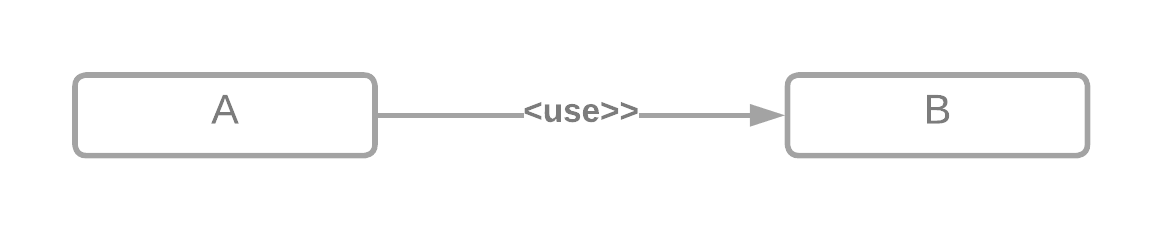
\includegraphics[width=1\textwidth]{./images/DIP - bad.png}
    \caption[Schlechte laut DIP Abhängigkeit]{Schlechte laut DIP Abhängigkeit}
    \label{fig:MVP}
\end{figure}


\begin{figure}[H]
    \centering
    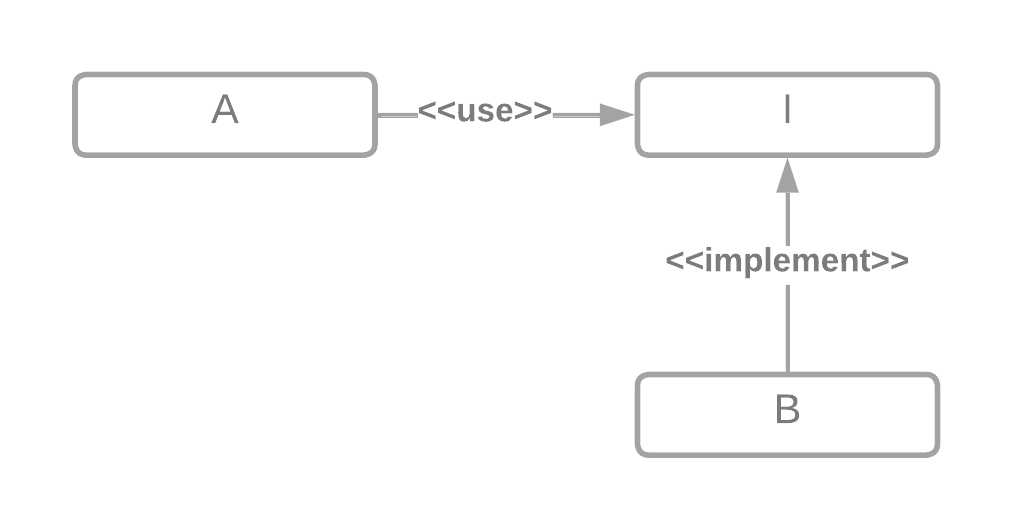
\includegraphics[width=1\textwidth]{./images/DIP - good.png}
    \caption[Gute laut DIP Abhängigkeit]{Gute laut DIP Abhängigkeit}
    \label{fig:MVP}
\end{figure}

% https://dewiki.de/Lexikon/Dependency-Inversion-Prinzip